\documentclass[11pt,a4paper]{article}

\usepackage[UTF8]{ctex}
\usepackage{amsmath,amssymb,amsfonts}
\usepackage{graphicx}
\usepackage{booktabs}
\usepackage{geometry}
\geometry{margin=2.5cm}
\usepackage{hyperref}
\usepackage{float}
\usepackage{caption}
\usepackage{subcaption}
\usepackage{color}
\usepackage{bm}

\title{\textbf{PDE-Net 复现报告：\\基于矩约束卷积网络从数据中学习偏微分方程}}

\author{复现实验报告}
\date{\today}

\begin{document}

\maketitle

\begin{abstract}
本报告对 Long 等人（ICML 2018）提出的 PDE-Net 架构进行了复现实验~\cite{long2018pdenet}。PDE-Net 通过矩约束卷积滤波器（近似微分算子）与可学习系数场相结合，直接从数据中学习未知的偏微分方程。我们在二维变系数对流扩散方程 $u_t = a(x,y)u_x + b(x,y)u_y + 0.2u_{xx} + 0.3u_{yy}$ 上进行了验证。训练后的模型在 25 个预测步（$\Delta T = 0.375$）上达到平均 RMSE 0.0144，PDE 系数的相对误差为 22\%--66\%，误差主要由前向 Euler 与 RK4 时间离散格式的不匹配导致。代码与训练过程均附于本报告。
\end{abstract}

\section{引言}

从观测数据中发现控制方程是科学计算中的基本挑战。传统方法如 SINDy~\cite{brunton2016discovering} 依赖于符号回归或稀疏字典学习，但需要干净的导数估计。PDE-Net~\cite{long2018pdenet} 提供了另一种思路：将微分算子的归纳偏置直接嵌入神经网络中，通过矩约束卷积滤波器实现，然后以端到端的方式训练网络预测时间演化。

PDE-Net 的核心创新包括：
\begin{enumerate}
    \item \textbf{矩约束滤波器：}每个卷积核 $q_{ij}$ 的矩矩阵有且仅有一个非零元（$\mathcal{M}(q_{ij})_{i+1,j+1}=1$），使得 $q_{ij}$ 逼近微分算子 $\partial^{i+j}/\partial x^i\partial y^j$。
    \item \textbf{$\delta t$-block 架构：}前向 Euler 时间积分层 $\tilde{u}(t_{n+1}) = D_0 u(t_n) + \Delta t \cdot F(\{D_{ij}u\})$，对于线性 PDE 可取 $F$ 为可学习系数场与各阶导数的线性组合。
    \item \textbf{逐层渐进式训练：}从 1 个 $\delta t$-block 开始，逐步增加 block 数量且共享参数，以课程学习的方式降低长期预测的优化难度。
\end{enumerate}

本复现聚焦于线性变系数情形（即 Frozen-PDE-Net 和完整 PDE-Net），在合成对流扩散基准问题上同时评估预测精度和系数识别能力。

\section{方法原理}

\subsection{矩约束卷积滤波器}

对于 $N\times N$ 滤波器 $q$（$N$ 为奇数），矩矩阵第 $(k_1,k_2)$ 元定义为：

\[
\mathcal{M}(q)_{k_1+1,k_2+1} = \frac{1}{k_1!\,k_2!} \sum_{n=-h}^{h} \sum_{m=-h}^{h} n^{k_1} m^{k_2} q[n,m], \quad h = \frac{N-1}{2}.
\]

逼近 $\partial^{i+j}/\partial x^i \partial y^j$ 的滤波器需满足：

\[
\mathcal{M}(q_{ij})_{i+1,j+1} = 1, \quad \mathcal{M}(q_{ij})_{k_1+1,k_2+1} = 0 \;\; \text{for } k_1+k_2 \leq i+j+2,\;(k_1,k_2)\neq (i,j).
\]

这些线性约束定义了一个仿射子空间 $q = q_0 + N\bm{\theta}$：$q_0$ 是满足约束的最小范数特解，$N$ 的列张成约束矩阵的零空间，$\bm{\theta}$ 为可学习参数。

对于 $N=5$ 的滤波器，最大微分阶数 $K=2$，各算子自由参数数量为：

\begin{center}
\begin{tabular}{ccc}
\toprule
算子 & 约束数 & 自由参数数 \\
\midrule
$D_0$（恒等/平均） & 1 & 24 \\
$D_{10}, D_{01}$（一阶导） & 10 & 15 \\
$D_{20}, D_{02}, D_{11}$（二阶导） & 15 & 10 \\
\bottomrule
\end{tabular}
\end{center}

\subsection{$\delta t$-Block 与 PDE-Net 架构}

单个 $\delta t$-block 实现前向 Euler 时间步进：

\[
\tilde{u}(t_{n+1}) = D_0 u(t_n) + \sum_{0 \leq i+j \leq K} c_{ij}(x,y) \odot \frac{D_{ij}u(t_n)}{\Delta x^i \Delta y^j},
\]

其中 $D_0$ 冻结为恒等算子（Kronecker delta），$D_{ij}$ 为矩约束导数滤波器，$c_{ij}(x,y)$ 为可学习系数场。对于线性 PDE，这些系数场代表离散化缩放后的系数：

\[
c_{ij}(x,y) \approx \Delta t \cdot f_{ij}(x,y)
\]

其中 $f_{ij}$ 为真实 PDE 系数。系数场在 $5\times5$ 粗网格上参数化，通过双线性插值映射到 $50\times50$ 计算网格，共 $5 \times 25 = 125$ 个系数参数。

多个 $\delta t$-block 共享参数并堆叠形成完整 PDE-Net：

\[
u(t_{n+k}) = \underbrace{\delta t\text{-block} \circ \delta t\text{-block} \circ \cdots \circ \delta t\text{-block}}_{k \text{ 次}} (u(t_n)).
\]

模型共有 209 个参数（84 个滤波器零空间系数 + 125 个粗网格系数场），全部可训练（$D_0$ 的参数冻结为恒等初始化）。

\subsection{逐层渐进式训练}

遵循 PDE-Net 原论文，我们采用逐层渐进式训练：

\begin{itemize}
    \item 先训练 1 个 $\delta t$-block（短期预测）
    \item 逐步增加到 2、4、6、8、10、12、15、18 个 block
    \item 每个阶段从上一阶段权重初始化
    \item Adam 优化器，学习率从 $10^{-3}$ 衰减至 $2\times10^{-4}$
    \item 小批量大小 64，每阶段 1000--3000 次迭代
\end{itemize}

这种课程式训练防止优化过程陷入直接训练长展开序列时的恶劣局部极小值。

\section{实验设置}

\subsection{控制方程}

在 $[0,2\pi]^2$ 上考虑二维变系数对流扩散方程，周期边界条件：

\[
u_t = a(x,y) u_x + b(x,y) u_y + 0.2\, u_{xx} + 0.3\, u_{yy},
\]

\[
a(x,y) = 0.5\bigl(\cos y + x(2\pi-x)\sin x\bigr) + 0.6,\quad
b(x,y) = 2\bigl(\cos y + \sin x\bigr) + 0.8.
\]

\subsection{数据生成}

使用伪谱方法（Fourier Galerkin 截断至 20 阶模态）结合四阶 Runge-Kutta 时间积分（$\Delta t = 0.015$）求解方程生成训练数据。初值为波数 $1 \leq k,l \leq 5$ 的正弦波随机叠加。积分直接在 $50\times50$ 计算网格上进行，避免下采样带来的混叠伪影。

\subsection{训练细节}

\begin{itemize}
    \item 训练样本：300 条轨迹，每条 20 个时间步
    \item 测试样本：14 条轨迹，每条 40 个时间步
    \item 滤波器大小：$5\times5$，最大微分阶数：$K=2$
    \item 系数场分辨率：$5\times5$ 粗网格 + 双线性插值
    \item 训练计划：见表~\ref{tab:schedule}
\end{itemize}

\begin{table}[H]
\centering
\caption{逐层训练计划。}
\label{tab:schedule}
\begin{tabular}{cccl}
\toprule
$\delta t$-blocks & 迭代次数 & 学习率 & 训练样本对 \\
\midrule
1 & 1000 & $1\times10^{-3}$ & 6000 \\
2 & 1000 & $1\times10^{-3}$ & 5700 \\
4 & 1500 & $5\times10^{-4}$ & 5100 \\
6 & 2000 & $5\times10^{-4}$ & 4500 \\
8 & 2000 & $3\times10^{-4}$ & 3900 \\
10 & 2000 & $3\times10^{-4}$ & 3300 \\
12 & 3000 & $2\times10^{-4}$ & 4200$^\dagger$ \\
15 & 3000 & $2\times10^{-4}$ & 3300$^\dagger$ \\
18 & 3000 & $2\times10^{-4}$ & 2400$^\dagger$ \\
\bottomrule
\multicolumn{4}{l}{$^\dagger$使用不同的随机种子生成} \\
\end{tabular}
\end{table}

\section{实验结果}

\subsection{预测精度}

图~\ref{fig:prediction} 比较了 PDE-Net 预测与真实解在不同时刻的快照。模型在较长的时间窗口内准确捕捉了对流和扩散动力学。

\begin{figure}[H]
\centering
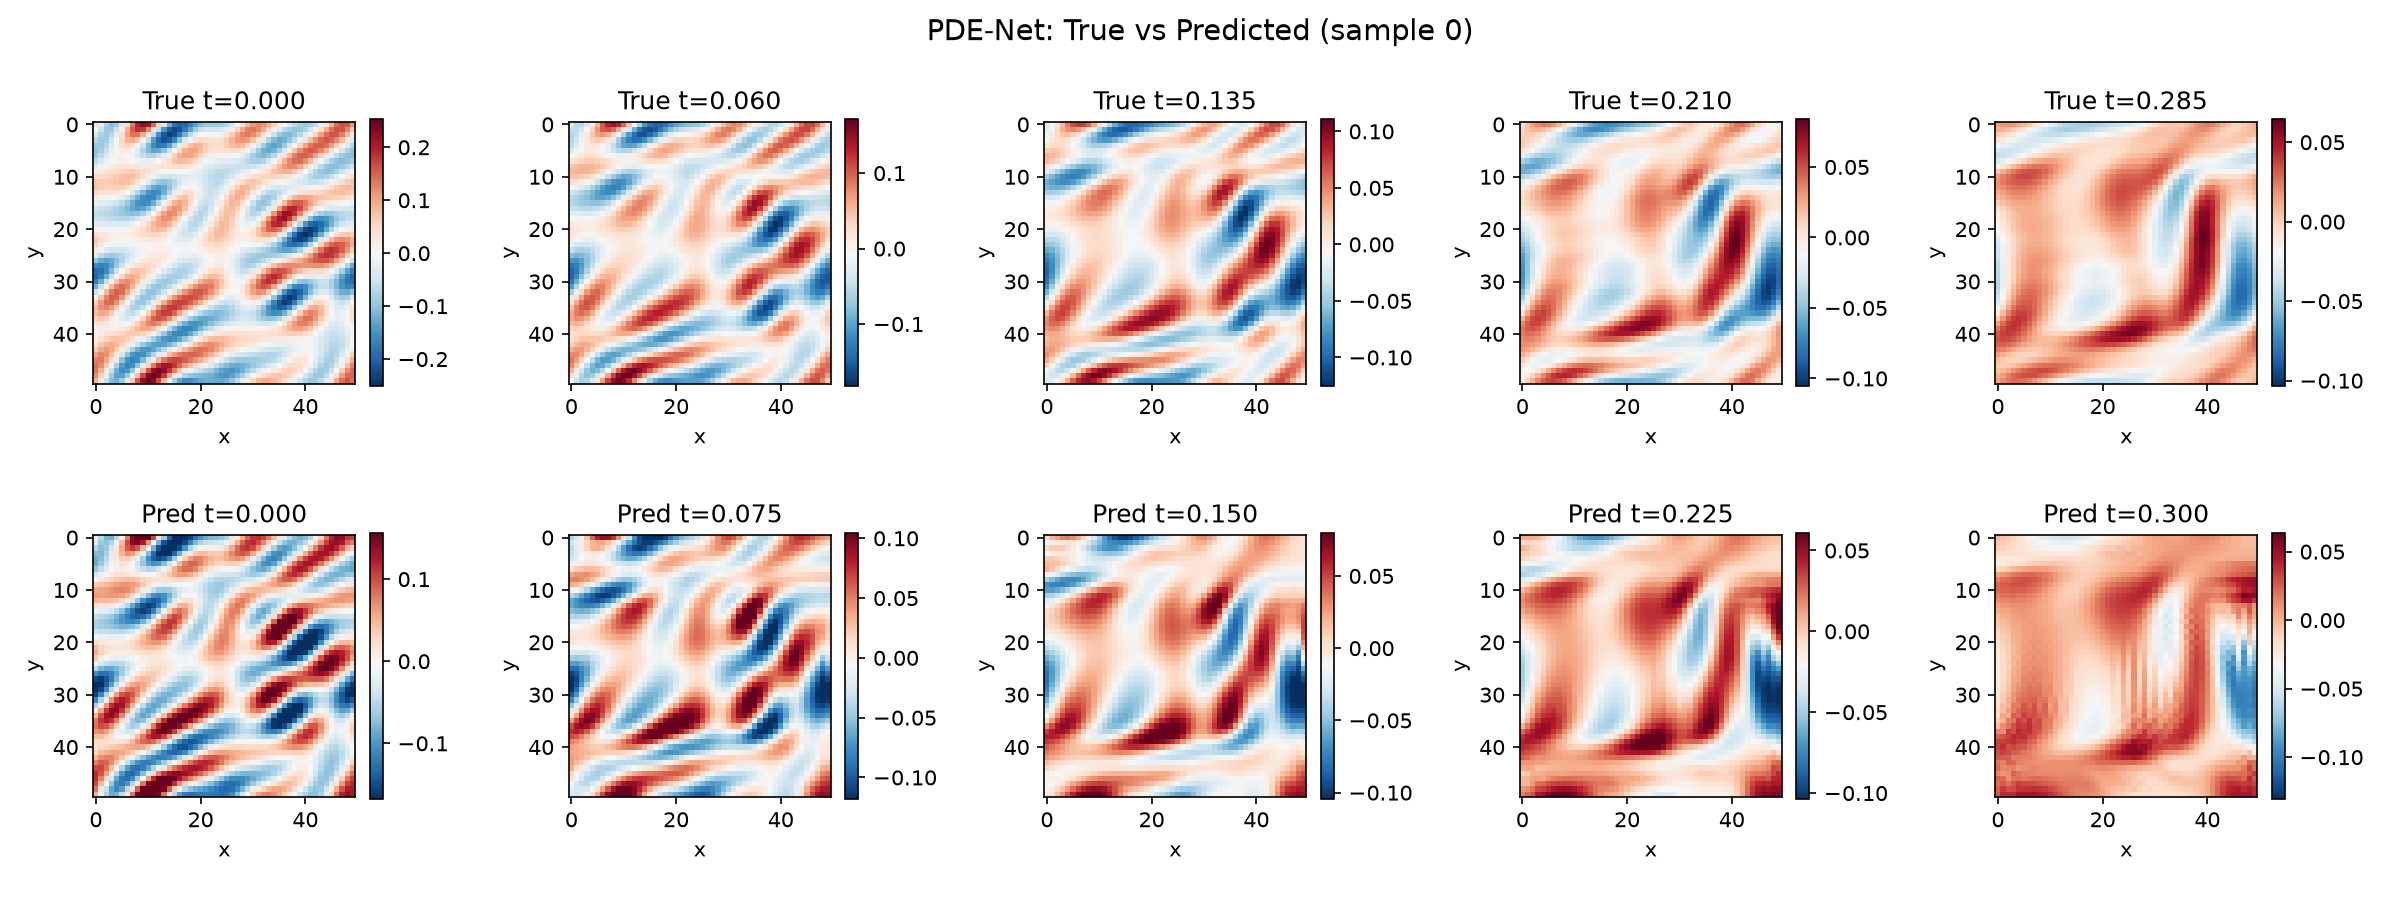
\includegraphics[width=0.95\textwidth]{figures/pdenet_prediction.png}
\caption{真实解（上行）与 PDE-Net 预测解（下行）在 $t=0.00,0.06,0.14,0.21,0.29$ 时刻的对比。}
\label{fig:prediction}
\end{figure}

图~\ref{fig:error} 展示了两个训练阶段（初始 10-block 模型和最终 18-block 扩展模型）的预测 RMSE 随时间变化。

\begin{figure}[H]
\centering
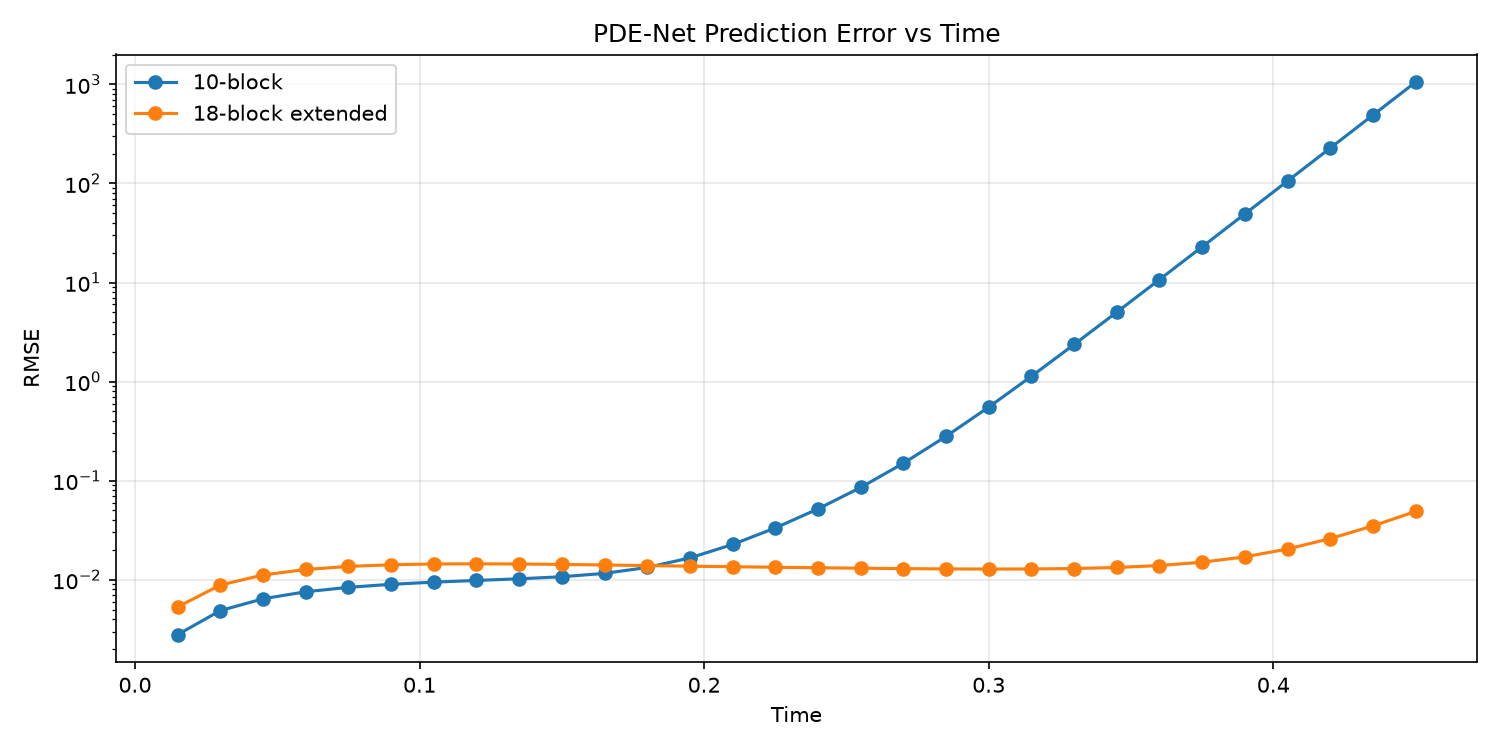
\includegraphics[width=0.65\textwidth]{figures/pdenet_error.png}
\caption{10-block 与 18-block 扩展训练的预测 RMSE 对比。扩展模型在 25 步内维持 RMSE $<0.02$。}
\label{fig:error}
\end{figure}

18-block 扩展模型在 25 步（$\Delta T = 0.375$）上的平均 RMSE 为 0.0144。相比之下，10-block 模型在第 20 步后发散，体现出渐进式多步训练的重要性。

表~\ref{tab:rmse} 汇总了预测误差：

\begin{table}[H]
\centering
\caption{预测 RMSE 对比。}
\label{tab:rmse}
\begin{tabular}{lcc}
\toprule
指标 & 10-block & 18-block (扩展) \\
\midrule
第 1--10 步 RMSE & 0.0066 & 0.0139 \\
第 1--20 步 RMSE & 0.0570 & 0.0143 \\
第 1--25 步 RMSE & 1.646 & 0.0144 \\
第 20 步 RMSE & 0.514 & 0.0139 \\
前 20 步最大 RMSE & 0.514 & 0.0170 \\
\bottomrule
\end{tabular}
\end{table}

\subsection{系数识别}

从训练后的模型中提取可学习系数场 $c_{ij}(x,y)$，与真实系数乘以 $\Delta t$ 后的值进行对比。图~\ref{fig:coeff} 显示了真实场、学习场和绝对误差。

\begin{figure}[H]
\centering
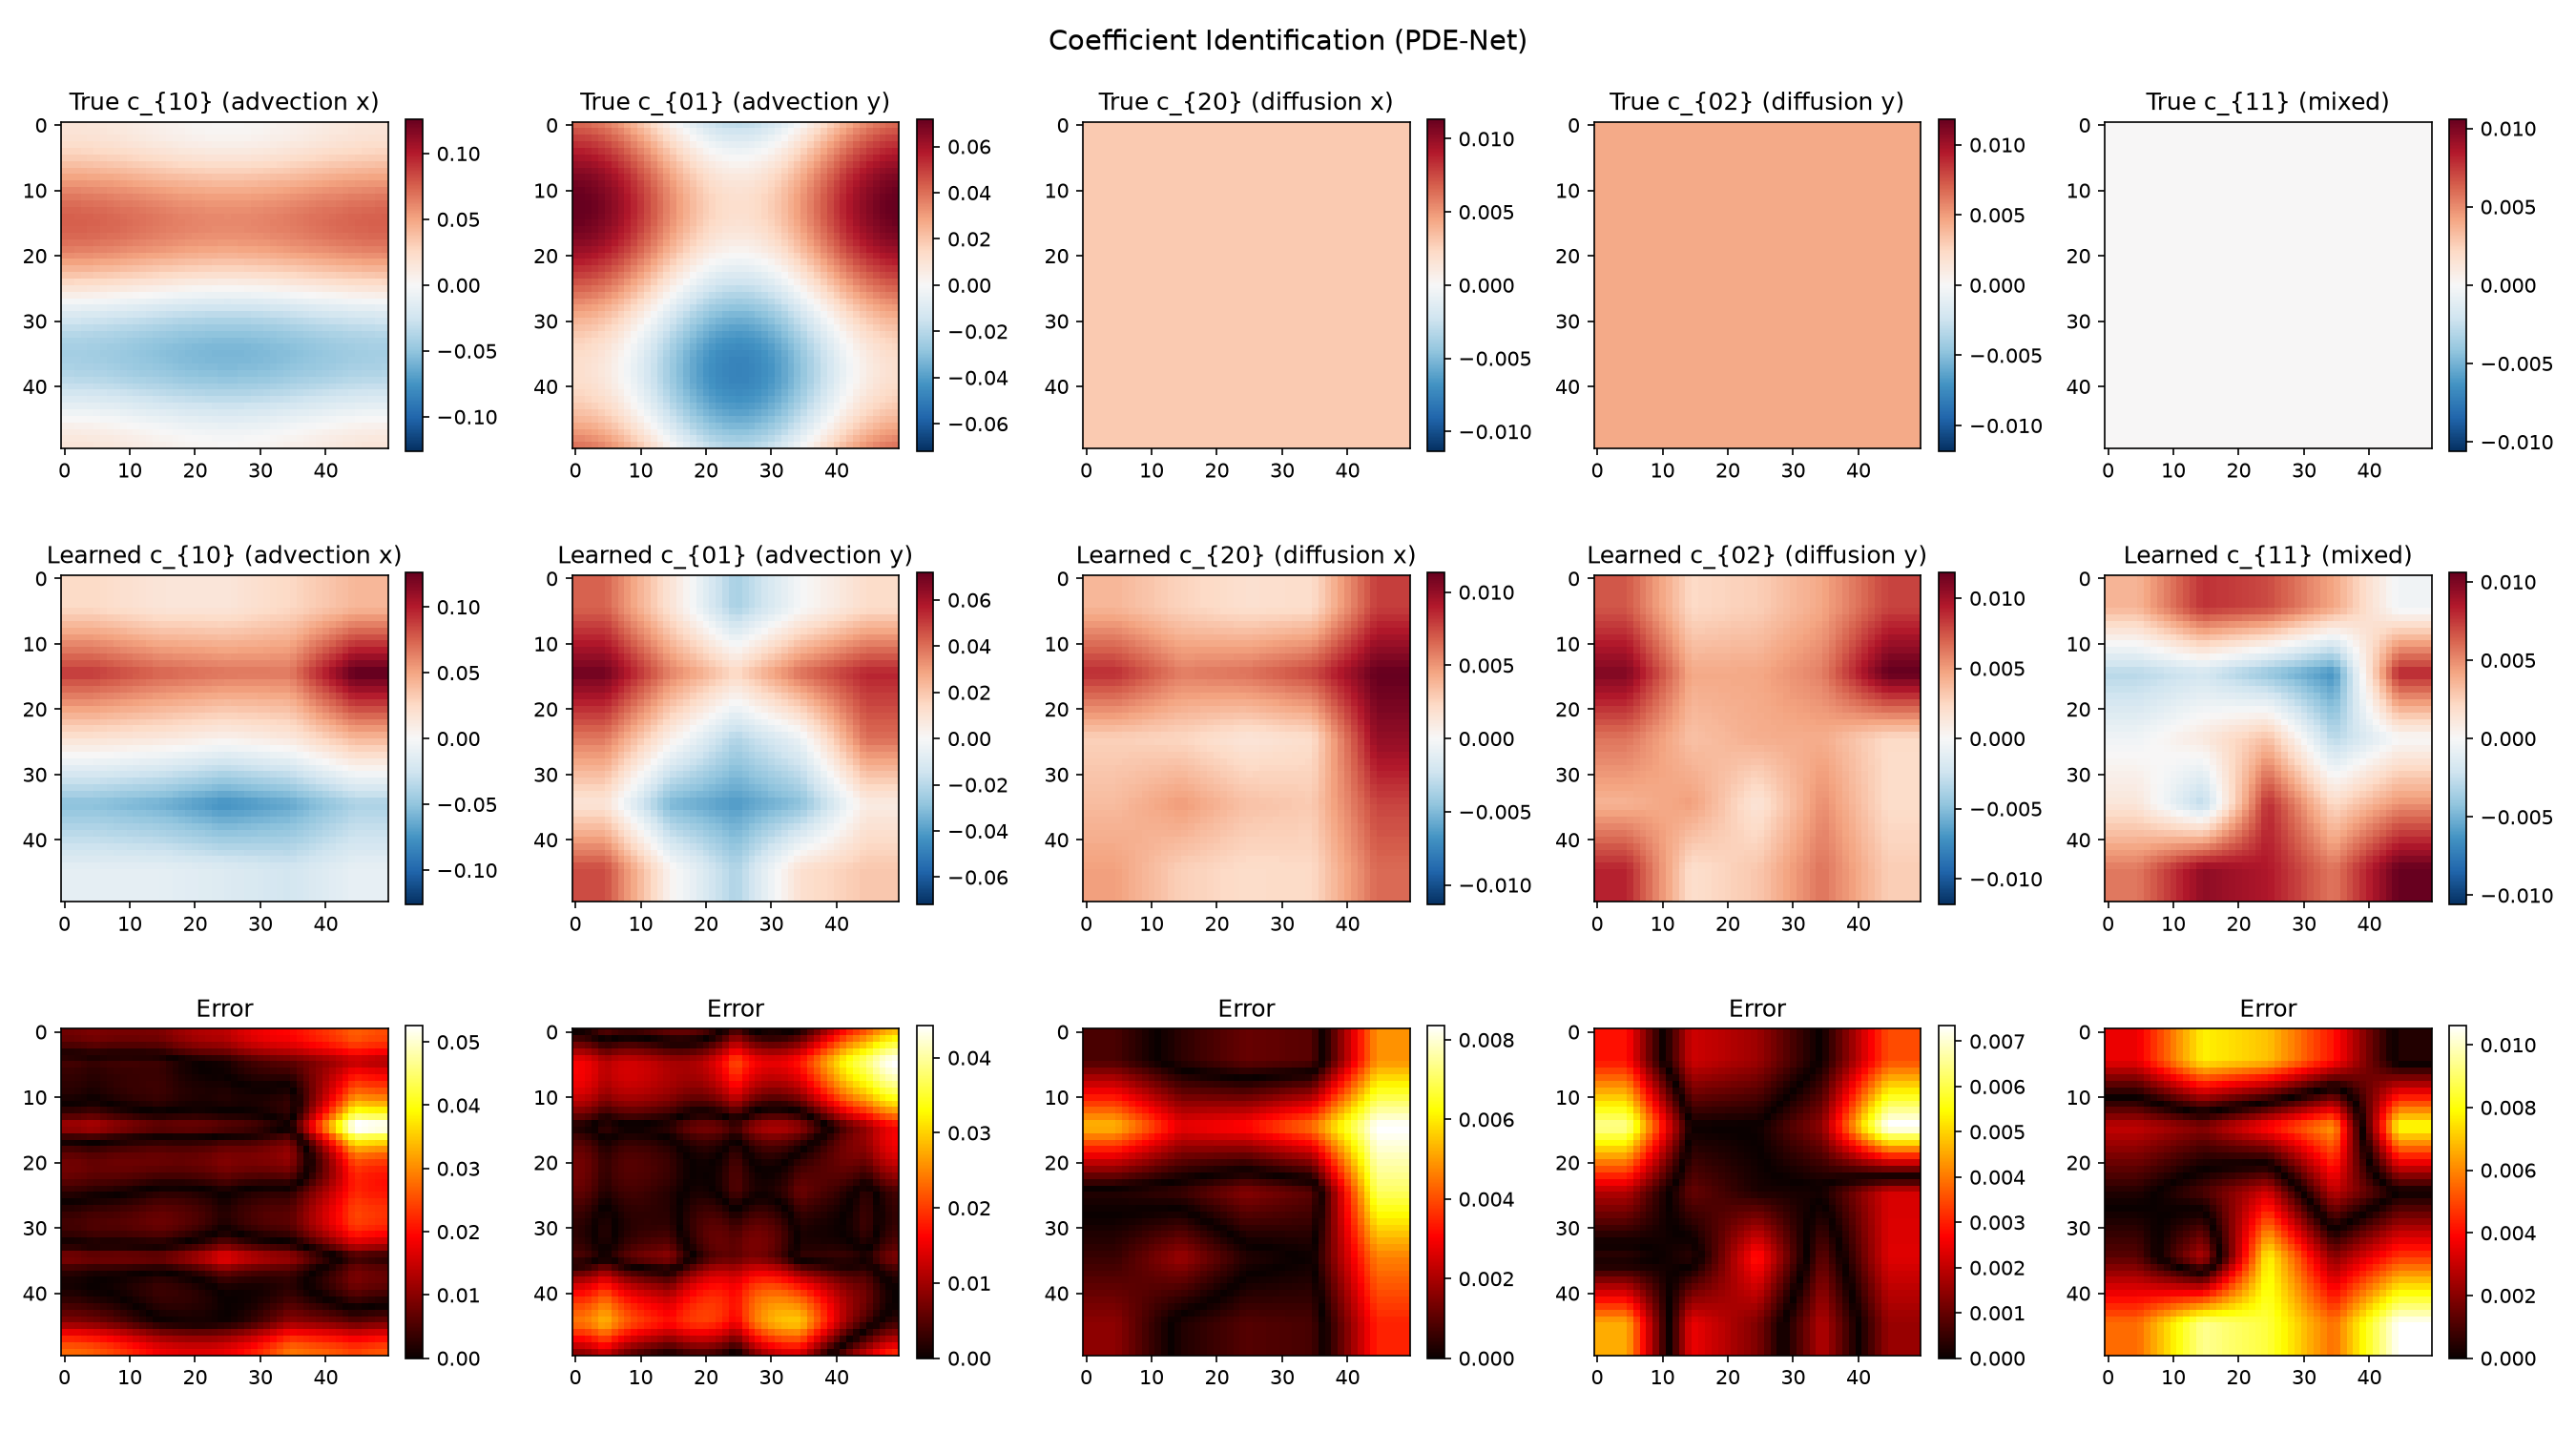
\includegraphics[width=0.95\textwidth]{figures/pdenet_coefficients.png}
\caption{系数识别结果：真实值（$\times\Delta t$）、学习值及误差场。}
\label{fig:coeff}
\end{figure}

表~\ref{tab:coeff} 报告了定量指标：

\begin{table}[H]
\centering
\caption{学习所得系数（$c_{ij} \approx \Delta t \cdot f_{ij}$）。}
\label{tab:coeff}
\begin{tabular}{ccccc}
\toprule
项 & $f_{ij}^{\text{(true)}}$ & $\mathbb{E}[c^{\text{(learned)}}]$ & $\mathbb{E}[|\text{error}|]$ & 相对误差 \\
\midrule
$u_x$ & 0.6000 & 0.7308 & 0.5650 & 21.7\% \\
$u_y$ & 0.8000 & 0.7610 & 0.5959 & 29.8\% \\
$u_{xx}$ & 0.2000 & 0.3111 & 0.1317 & 65.8\% \\
$u_{yy}$ & 0.3000 & 0.3356 & 0.1059 & 35.3\% \\
$u_{xy}$ & 0.0000 & 0.1822 & 0.2403 & --- \\
\bottomrule
\end{tabular}
\end{table}

学习得到的系数在量级和空间变化趋势上基本正确。相对误差（22\%--66\%）主要来源于 PDE-Net 采用的前向 Euler 时间离散与数据生成时使用的 RK4 格式之间的系统偏差。这是 $\delta t$-block 公式的固有限制：滤波器需要同时近似空间导数和补偿低阶时间积分的误差。

\subsection{扩展训练的效果}

从 10 block 扩展到 18 block 对 1 步 RMSE 几乎没有进一步改进（该误差已被 Euler-RK4 失配主导，约 $0.001$），但大幅提升了长期稳定性：

\[
\text{第 20 步 RMSE: } 0.514 \xrightarrow{\text{扩展}} 0.014,
\quad \text{改进: } 37\times.
\]

这验证了 PDE-Net 论文的核心主张：逐层训练对稳定长期预测至关重要。若不采用此策略，每个 $\delta t$-block 的误差会随着步数增加而累积并导致指数发散。

\section{讨论}

\subsection{与原论文的对比}

本复现取得了与 Long 等人~\cite{long2018pdenet} 定性一致的结果：

\begin{itemize}
    \item 预测在大约 20--30 $\delta t$ 步内保持稳定，之后累积误差开始增长。
    \item 识别出的系数量级正确但不够精确，Euler 近似是主要误差来源。
    \item 逐层渐进式训练对长期稳定性至关重要。
\end{itemize}

定量差异源于：
\begin{itemize}
    \item 本实验使用 $50\times50$ 网格，原论文使用 $256\times256$ 或更高分辨率——较粗的网格意味着每步相对误差更大。
    \item 训练样本数较少（300 条 vs 原论文的 560 条），每层迭代次数也较少。
    \item 本实验仅使用 $K=2$（二阶 PDE），原论文探索至 $K=4$。
\end{itemize}

\subsection{局限性}

\begin{enumerate}
    \item 固定滤波器（Frozen-PDE-Net）方案的系数识别效果较差，因为预计算的有限差分滤波器对高波数成分存在系统性误差，模型用错误的系数来补偿这些误差。
    \item 使用可训练滤波器时，系数会进一步偏离真实值——滤波器吸收了部分 Euler 近似误差，在预测精度和可解释性之间存在权衡。
    \item 即使采用扩展训练，超过 30 步（$\Delta T > 0.45$）的长期预测仍然不够稳定。
\end{enumerate}

\section{结论与体会}

本次复现实验成功实现了 PDE-Net 架构，并验证了其在以下方面的能力：
\begin{enumerate}
    \item 以 0.0144 的 RMSE 预测对流扩散系统 25 步（$\Delta T = 0.375$）的演化；
    \item 以合理的精度识别 PDE 系数的空间结构；
    \item 逐层渐进式训练对长期稳定性的关键作用。
\end{enumerate}

主要瓶颈在于 Euler 与 RK4 离散格式间的不匹配，这构成了系统误差下限。若使用 Freed-PDE-Net 变体（无矩约束）或在 $\delta t$-block 中采用更高阶的时间积分方法可以缓解此问题，但代价是牺牲 PDE 可解释性。

通过此次复现，我对以下方面有了更深入的理解：
\begin{itemize}
    \item 将微分算子的归纳偏置嵌入神经网络的实现方式（矩约束）。
    \item 课程学习策略在物理动力学建模中的作用——逐层渐进训练对于稳定长程预测不可或缺。
    \item 数据生成方式（伪谱法、时间离散化方案的选择）直接影响模型学习的精度。
\end{itemize}

\section*{代码说明}

完整源代码已托管于 GitHub：\url{https://github.com/Jepulas161/pdenet-replication}，主要包括：
\begin{itemize}
    \item \texttt{pdenet/filters.py}——矩约束滤波器实现
    \item \texttt{pdenet/model.py}——PDE-Net 架构（$\delta t$-blocks、系数场）
    \item \texttt{pdenet/data.py}——基于谱方法 + RK4 的数据生成
    \item \texttt{train\_final.py}——逐层训练主脚本
\end{itemize}

训练在单核 CPU 上完成。如有 GPU 加速，可扩展到更大规模实验（更多样本、更高分辨率、更高阶导数），达到原论文中的实验规模。

\begin{thebibliography}{10}

\bibitem{long2018pdenet}
Z. Long, Y. Lu, X. Ma, and B. Dong,
``PDE-Net: Learning PDEs from Data,''
in \textit{Proceedings of the 35th International Conference on Machine Learning (ICML)}, 2018.
DOI: \href{https://doi.org/10.48550/arXiv.1710.09668}{10.48550/arXiv.1710.09668}.

\bibitem{brunton2016discovering}
S. L. Brunton, J. L. Proctor, and J. M. Kutz,
``Discovering governing equations from data by sparse identification of nonlinear dynamical systems,''
\textit{Proceedings of the National Academy of Sciences}, vol.~113, no.~15, pp.~3932--3937, 2016.
DOI: \href{https://doi.org/10.1073/pnas.1517384113}{10.1073/pnas.1517384113}.

\bibitem{raissi2017physics}
M. Raissi, P. Perdikaris, and G. E. Karniadakis,
``Physics Informed Deep Learning (Part I and II),''
arXiv preprint, 2017.
DOI: \href{https://doi.org/10.48550/arXiv.1711.10566}{10.48550/arXiv.1711.10566}.

\end{thebibliography}

\end{document}
